\begin{frame}{Diagram elements - Twobody Hamiltonian}
    \note{Filename: diagram\_hamiltonian02.tex}

    \renewcommand{\figurename}{Level}

    \begin{figure}
    \centering
    \parbox{0.30\textwidth}{
            \centering
            
\includegraphics[scale=0.45]{graphics/v1}
            \caption{-2}
        }\quad
        \parbox{0.30\textwidth}{
            \centering
            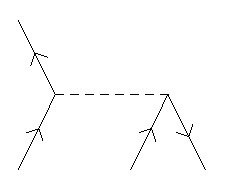
\includegraphics[scale=0.45]{graphics/v2}
            \caption{-1}
        }\quad
        \parbox{0.30\textwidth}{
            \centering
            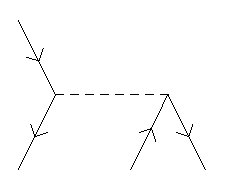
\includegraphics[scale=0.45]{graphics/v3}
            \caption{-1}
        }
    \end{figure}

    \begin{figure}
    \centering
    \parbox{0.30\textwidth}{
            \centering
            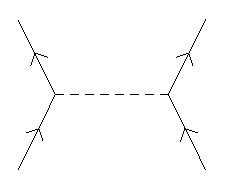
\includegraphics[scale=0.45]{graphics/v4}
            \caption{0}
        }\quad
        \parbox{0.30\textwidth}{
            \centering
            
\includegraphics[scale=0.45]{graphics/v5}
            \caption{0}
        }\quad
        \parbox{0.30\textwidth}{
            \centering
            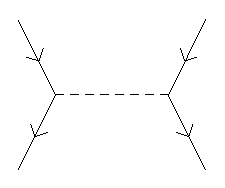
\includegraphics[scale=0.45]{graphics/v6}
            \caption{0}
        }
    \end{figure}

    \begin{figure}
    \centering
    \parbox{0.30\textwidth}{
            \centering
            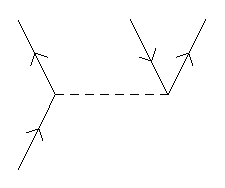
\includegraphics[scale=0.45]{graphics/v7}
            \caption{+1}
        }\quad
        \parbox{0.30\textwidth}{
            \centering
            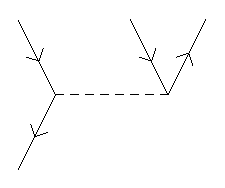
\includegraphics[scale=0.45]{graphics/v8}
            \caption{+1}
        }\quad
        \parbox{0.30\textwidth}{
            \centering
            
\includegraphics[scale=0.45]{graphics/v9}
            \caption{+2}
        }
    \end{figure}

\end{frame}

    
